\documentclass[10pt]{IEEEtran}
\pdfoutput=1

\usepackage{graphicx}
\usepackage{hyperref}
\usepackage[utf8]{inputenc}
\usepackage{listings}
\usepackage[table]{xcolor}
\usepackage{pdfpages}

\hypersetup{colorlinks=true,citecolor=[rgb]{0,0.4,0}}


\title{Twitter Sentiment Diffusion}
\author{Matthias Baetens (s142485) \& Karol Dzitkowski (s142246)}

\begin{document}
\maketitle

\begin{abstract}
We build software to evaluate the most important features of a Tweet and their influence on the number of retweets. We used both the standard Tweet-features as well as a calculated value for the sentiment of a Tweet. We used a number of different Machine Learning models and algorithms including neural networks to compare the performance of these methods. Our system can be dynamically accesed using a webpage which is able to download new Tweets, run the different Machine Learning algorithms, perform analysis and generate relevant charts. 
\end{abstract}

\section{Introduction}
One of the most important features to measure the popularity of a Tweet is the number of retweets. Next to the number of favorites, which counts how much people like a post, the number of retweets counts the number of times another user reshared the post, and thus wants to identify himself with the post and wants to share it with other. This means it is very interesting to research the possibility to optimize Tweets in order to get more retweets and to spread your message. 

Tweets not only consists of the message itself: they have a huge amount of metadata: 
\begin{itemize}
	\item The time of creation of the Tweet and the user profile.
	\item The location. 
	\item Whether there is a URL, an image, ...
	\item The hashtags (and the amount of hashtags)
	\item The number of followers and friends
	\item ...
\end{itemize}

Using the text, it is possible to calculate a certain sentiment for each Tweet; which can also be seen as a feature of the Tweet. For example: a Tweet with ``awesome day'' will have a more positive sentiment value than a tweet with ``bad day''.

We concentrated on building a basic system that downloads Tweets relevant to a certain query, calculate a sentiment and save them to a database. We implemented 6 different Machine Learning algorithms: 4 for classification and 2 for regression. The classification is used to classify tweets in a certain sentiment class using the favorite count of the Tweet, followers count of the user, retweet count of the Tweet and age of the Tweet as an input. The regression algorithms are used to predict the number of retweets based on the favorite count of the Tweet, followers count of the user, calculated word sentiment and the age of the Tweet. The results can be accessed through a website, which is implemented using Django.

\section{Related work}

In Suh et. al. \cite{want_to_be_retweeted} the authors tried to quantitatively identify factors that are associated with retweeting. They split up the factors in 2 classes of features: content features and contextual features and found that for the content features URLs and hashtags seemed to have an influence on the retweet rate and for the contextual features, the number of followers and followees and the age of the account seemed to have an influence. 

Dan Zarrella \cite{science_of_retweets} found that users with more followers indeed get more retweets, but there are certain users without a lot of followers who get a lot of retweets, so the content of the tweets must be of some importance too. He also found that there were significantly more links in the retweets than in the tweets (56.69 \% versus 18.96 \%). Novelty (``newness'' of the ideas and information presented) also turns out to be an important feature. The late afternoon until night (3 PM until midnight) is the most popular time to retweet. 

\section{Software}

In Figure \ref{software1} you can see a coarse overview of our software. In this section we will describe the different parts of our software and what their respective functionalities are.

\begin{figure}[h!]
\begin{center}
	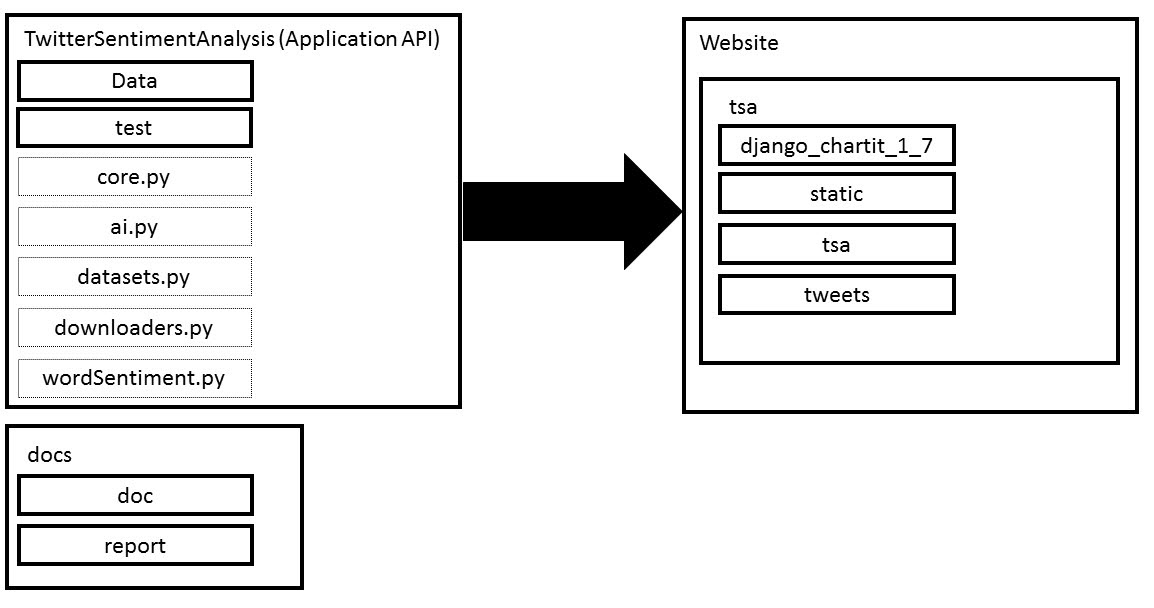
\includegraphics[width=0.45\textwidth]{images/software}
\caption{Overview of the built software. \label{software1}}
\end{center}
\end{figure}
\subsection{The main logic/API (TwitterSentimentAnalysis)}

The \emph{TwitterSentimentAnalysis}-package contains all the logic and processing of data of our application.

\subsubsection{Data}

This folder contains the data used in the application: 
\begin{itemize}
	\item corpus.csv: the downloaded file containing records with the topics, sentiment rating and Tweet-id specified.
	\item words.txt: the AFINN wordlist containing different words and their sentiment value. This file is used to calculate the sentiment of our Tweets.
	\item ai-folder: contains the saved (and trained) Artificial Intelligences used on the website.
\end{itemize}

\subsubsection{test}

This folder contains all the tests written to test the logical part of our software.

\subsubsection{core.py}

core.py takes care of all initializing and sets up connections to Twitter and our database. It reads the necessary parameters from the \emph{configuration.cfg}-file.

\subsubsection{ai.py}

This file contains all the Machine Learning algorithms used to predict the sentiment and the retweet count. We have implemented 6 different Machine Learning algorithms, 4 to classify the Tweets in a certain sentiment class and 2 to predict the retweet count.
Classification:
\begin{itemize}
	\item MultiClassClassificationNeuralNetwork: uses the Pybrain library \cite{pybrain} to construct an Artifical Neural Network with 2 hidden layers and 4 and 9 neurons in the first and second layer respectively. 
	\item SimpleClassificationNeuralNetwork: uses the native Pybrain NNclassifier class from Pybrain tools to set up an Artificial Neural Network for classification. 
	\item NaiveBayesClassifier: this class implements Machine Learning using the Naive Bayes Classifier from the NLTK package \cite{nltk}. 
	\item MaxEntropyClassifier: this class implements Machine Learning using the Maximum Entropy classifier from the NLTK package. 
\end{itemize}

Regression:
\begin{itemize}
	\item SimpleRegressionNeuralNetwork: uses the native Pybrain NNregression class from Pybrain tools to set up an Artificial Neural Network for regression 
	\item LinearRegression: this class implements regression using the LinearRegression class from the scikit-package \cite{sklearn}.
\end{itemize}

All the models can be trained, evaluated (with or without using crossvalidation), saved and loaded.

\subsubsection{datasets.py}

These classes take care of the data preprocessing for the regression and classification problems. 
The sentiment of a Tweet gets calculated using the wordlist the following way: we search for every word in the Tweet if it is part of the wordlist and if it is, it is added to the total sum. This sum is divided by the number of words in the Tweet that are in the wordlist. This renders a result between -5 and 5. The result is then scaled to a value between 0 and 4. If there is a manual grade available (positive or negative, only for the Tweets in the downloaded file), the wordsentiment gets multiplied by 1 or -1, depending if the manual grade is positive or negative. Else, it just takes the sign it had in the beginning. This way we get 9 classes of sentiment, ranging from -4 (highly negative) to +4 (highly positive). 
For the classification in the different word sentiment classes the following features of the Tweets are used:
\begin{itemize}
	\item Favorite count: the number of times a Tweet is favorited.
	\item Followers count: the number of followers the user who tweeted has.
	\item Retweet count: the number of times the Tweet has been retweeted.
	\item Age of the tweet: how old the Tweet is.
\end{itemize}

For the regression of the retweet count the following features of the Tweets are used:
\begin{itemize}
	\item Favorite count: the number of times a Tweet is favorited.
	\item Followers count: the number of followers the user who tweeted has.
	\item Word sentiment: the word sentiment calculated as specified above.
	\item Age of the tweet: how old the Tweet is.
\end{itemize}

\subsubsection{downloaders.py}

This class takes care of downloading the Tweets using Tweepy \cite{tweepy}. It takes into account the rate limits of the Twitter API so our downloads do not get blocked. Tweets are saved to a specified MongoDB table using Pymongo \cite{pymongo}, using a tag as a label when we save. This class also implements the possibility to undersample the data: because the majority of the Tweets has a sentiment of 0, the Artificial Intelligence is trained in a wrong way (a classifier which predicts all tweets to be 0 will have a very low training error and maybe even test error, although we this classifier will be useless). The undersampling  will undersample data with a sentiment close to 0 (standard treshold is set to be 0.4). 

\subsubsection{wordSentiment.py}

In the WordSentimentAnalyzer class the sentiment gets calculated like stated above using the AFINN lexicon \cite{AFINN}. 

\subsection{The website (site)}

This folder contains all the code for running the site. We included the django\_chartit\_1\_7 package, because it had to be adapted in order to work together with package we wanted to use for our charts. This package is thus not completely written by ourselves, but adapted from \cite{django}. It contains all the logic of the different views of our site: home, analysis, statistics and contact. 

\section{Results}

In this section we will talk about the results we had using our software. The error rates the different Machine Learning algorithms obtain are gathered in Table \ref{tableclassification} for the classification of the sentiment and Table \ref{tableregression} for the prediction of the retweet count using regression. 

\begin{table}[h!]
	\centering
		\begin{tabular}{ | >{\bfseries}l || c | c |}
		\hline
		& \emph{MultiClassClassification} & \emph{SimpleClassification} \\ 
		& \emph{Neural Network} & \emph{Neural Network} \\
		\hline
		\hline
		Error rate & 21.07 & 19.63 \\ 
		\hline  
		&  \emph{Naive Bayes Classifier} &  \emph{Maximum Entropy Classifier} \\
		\hline
		\hline
		Error rate &  25.96 & 22.97 \\
		\hline
		\end{tabular}
    \caption{Error rates of the Machine Learning algorithms for classification.}
    \label{tableclassification}
\end{table} 

\begin{table}[h]
	\centering
		\begin{tabular}{ | >{\bfseries}l || c | c |}
		\hline
		&  \emph{Linear Regression} & \emph{SimpleRegression Neural Network} \\ 
		\hline
		\hline
		Error rate & 38.77 & 11.11 \\ 
		\hline  
		\end{tabular}
    \caption{Error rates of the Machine Learning algorithms for regression.}
    \label{tableregression}
\end{table} 

We can see that the Artificial Neural Networks perform the best for classification: the smallest error rate is obtained by the SimpleClassification Neural Network using the Pybrain tools, obtaining an error rate just under 20\%. We can see in the results though that the Neural Networks also mainly predict zero sentiments, which are not the results we hoped for. This problem should be solved in any future work on this topic: we could implement more sophisticated tweet filtering to generate train data and we could make a better system to calculate the actual sentiment. 

The prediction of the retweet count is our best performing part: the Neural Network is able to perform regression to predict this feature, obtaining an error rate of just over 11 percent. We can see the Linear Regression performs really poor. Same comments apply to the regression: our data can be preprocessed in a better way and the sentiment calculation could be more complex. 

Using the website we were able to generate some results. One of the graphs we looked at was the number of followers versus the number of retweets, to see if more followers automatically results in more retweets. The graph can be seen in Figure \ref{result1} (predicted using Linear Regression). We can see some peaks in number of retweets, but they occur as often for a smaller number of followers as for larger numbers. Our predicted retweet rate remains pretty small; it doesn't really predict any peaks. This is difficult, because the peaks appear to be pretty random and large compared to the ``normal'' amount of retweets. 

\begin{figure}[h!]
\begin{center}
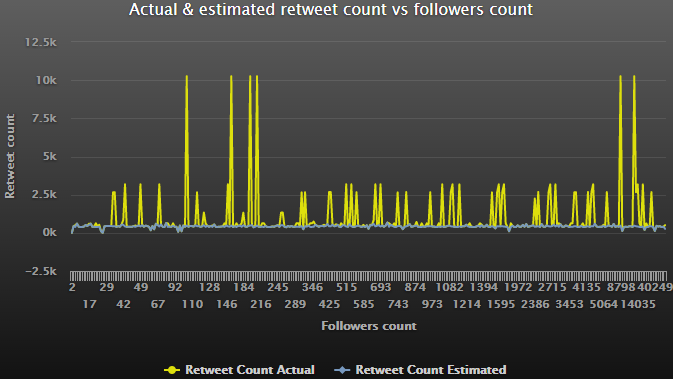
\includegraphics[width=0.4\textwidth]{images/giving_tuesday_linear_regression_followers_vs_retweet}
\caption{Number of followers vs actual and predicted retweet count. \label{result1}}
\end{center}
\end{figure}

It is also interesting to look at the time of the day and the day of the week for both the number of retweets and the performance of our predictions. In Figure \ref{result2} and Figure \ref{result3} these results can be seen. 

\begin{figure}[h!]
\begin{center}
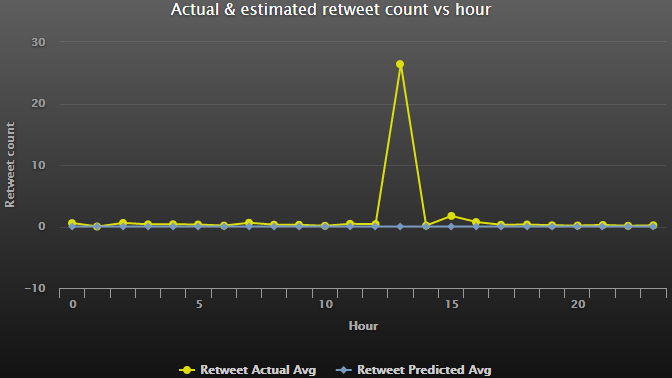
\includegraphics[width=0.4\textwidth]{images/srnn_hour_vs_retweet}
\caption{Number of retweets vs hour of the day. \label{result2}}
\end{center}
\end{figure}

\begin{figure}[h!]
\begin{center}
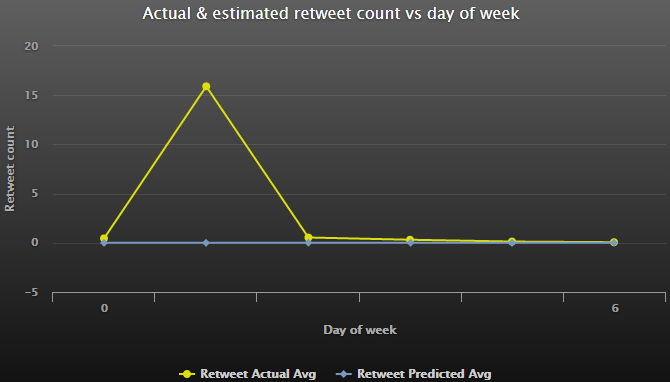
\includegraphics[width=0.4\textwidth]{images/srnn_day_of_week_vs_retweet}
\caption{Number of retweets vs day of the week. \label{result3}}
\end{center}
\end{figure}

We can see there is a peak in retweets on the second day of the week and between 12 and 14 o' clock. We think this peak is due to the lunch pause; people just have one hour of spare time wherein they can Tweet. Again, our predictions have difficulties to keep up with this peaks. 

\section{Conclusion}

We delivered a basic system which is able to download Tweets, uses Machine Learning to classify the Tweets in different sentiment classes and to predict the retweet count using regression and which shows the results on a webpage. There are a lot of extensions and improvements possible in our system, but because of the flexibility of our system, this is possible. One of the most important things for future work is the improvement of the sentiment calculation: we could also use Machine Learning to calculate the sentiment value, taking into account the context wherein the words occurs; we could for example give different sentiment values to the words ``bad'' and ``really bad''. Another possibility to improve the sentiment calculation could be to use more wordlists and compare their performance. We could also improve our results by using our API to analyze a larger database instead of just using the website for our results. Our data preprocessing scheme could also be improved to include more advanced ways of dealing with the large sentiment zero class. Some of the features we used for Machine Learning can also be transformed to improve the performance: for example, the number of followers or retweets can quickly become a large number for popular accounts (we think of millions of followers and thousands of retweets). Taking the square root or the log of these values could improve the results of our Artificial Intelligence. We think this project is a good basis for further exploration of this field and a lot of interesting results can emerge, using the right techniques. 

\bibliographystyle{IEEEtran}
\bibliography{lyngby}

\clearpage
\end{document}